\documentclass[a4paper,10pt]{article}
\usepackage[utf8]{inputenc}
\usepackage{graphicx}
\usepackage{float}

\begin{document}

\section*{Trabalho de Programação para Dispositivos Móveis}

O trabalho consiste em criar uma estrutura que une pessoas com trocado a pessoas que precisam de troco. A data limite para entrega é até dia \textbf{04/06}.
Considerações:
\begin{itemize}
  \item O trabalho deve ser feito tendo como base o SDK 19 (Kit Kat);
  \item Na tela \textbf{Tenho/Preciso de Troco} após clicar em enviar deve aparecer um Toast informando o valor total solicitado e quantidade solicitada para cada nota/moeda; e
  \item O fluxo da aplicação deve ser \textbf{Tela de Cadastro} $>$ \textbf{Tela Inicial} $>$ \textbf{Tela de Tenho/Preciso de Troco} $>$ \textbf{Tela Inicial}.
\end{itemize}

As telas de cadastro e de troco \textbf{DEVEM SER VALIDADAS}:
\begin{itemize}
 \item Não deve ser permitido avançar sem preencher o cadastro todo; e
 \item Valores negativos para notas/moedas não são permitidos.
\end{itemize}

\newpage

\subsection*{Tela de Cadastro}

Essa tela será a primeira tela que o usuário deve ver se não tiver feito o cadastro no aplicativo. Ao completar o cadastro, o mesmo será salvo no banco de dados do aplicativo e essa tela não será exibida novamente.

\begin{figure}[H]
    \centering
    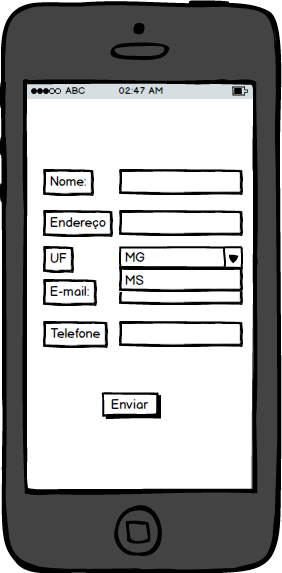
\includegraphics[scale=0.7]{t2_img/Cadastro.png}
\end{figure}

\newpage

\subsection*{Tela Inicial}

Tela para permitir que o usuário selecionar se ele possui troco ou se ele precisa de troco, sendo essa tela utilizada apenas para diferenciar como será salvo no banco as informações obtidas pela próxima tela.

\begin{figure}[H]
    \centering
    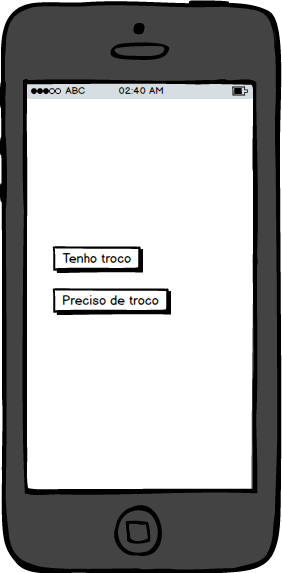
\includegraphics[scale=0.7]{t2_img/Inicial.png}
\end{figure}

\newpage

\subsection*{Tela Preciso de Troco}

Nessa tela serão informados os valores para o troco que o usuário necessita. Ao concluir, as informações serão gravadas no banco e será exibido uma mensagem contendo o valor total solicitado e os valores para cada moeda/nota.

\begin{figure}[H]
    \centering
    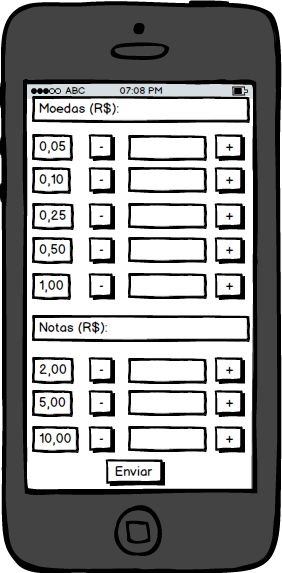
\includegraphics[scale=0.7]{t2_img/Preciso.png}
\end{figure}

\newpage

\subsection*{Tela Tenho Troco}

Nessa tela será exibido uma lista com todos os pedidos de troco gravados no banco e, ao clicar em um troco exibido, deve marcar o troco como realizado. Ao clicar em "Histórico", será exibido a lista com todos os pedidos de troco que o usuário atendeu.

\begin{figure}[H]
    \centering
    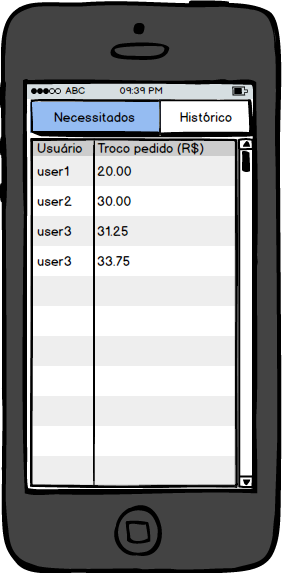
\includegraphics[scale=0.7]{t2_img/Tenho.png}
\end{figure}

\end{document}
